\section{Estensioni e originalità}
\label{cap:extensions-and-originalities}

\noindent Oltre alle tre implementazioni richieste dalla consegna
dell'homework, abbiamo deciso di esplorare qualche altro algoritmo per il problema del commesso viaggiatore negli spazi metrici.

\subsection{Farthest Insertion}
\label{sec:farthest-insertion}

\noindent Farthest Insertion è una delle euristiche impiegabili per la
risoluzione di Metric-TSP in modo approssimato. Questa euristica è
molto simile a Closest Insertion (si veda
\ref{sec:closest-insertion}), infatti differisce da essa solo per la
selezione del vertice $k$ da inserire nel circuito parziale $C$. In particolare, in Farthest Insertion viene scelto il vertice $k$
non presente nel circuito $C$ che massimizza $\delta (k, C)$.

\subsubsection{Implementazione}

\noindent Il codice è sostanzialmente identico a quello riportato nel
listato \ref{listing:closest-insertion}, con la differenza che per
Farthest Insertion si effettua la scelta del nuovo nodo con:

\begin{center}
\mintinline{c++}{utils::select_new_k_maximize(not_visited, circuit, get_distance)}
\end{center}

% \subsubsection{Approssimazione}

% \noindent Questa euristica permette di trovare una soluzione
% $\log(n)$-approssimata, ma è possibile dimostrare che il fattore di
% approssimazione può essere ulteriormente abbassato fino ad avere una
% soluzione $2$-approssimata.\\

\noindent I risultati che abbiamo ottenuto con Farthest Insertionsono
illustrati dal grafico \ref{fig:farthest-insertion-accuracy-error}.\\

\begin{figure}[H]
    \centering

    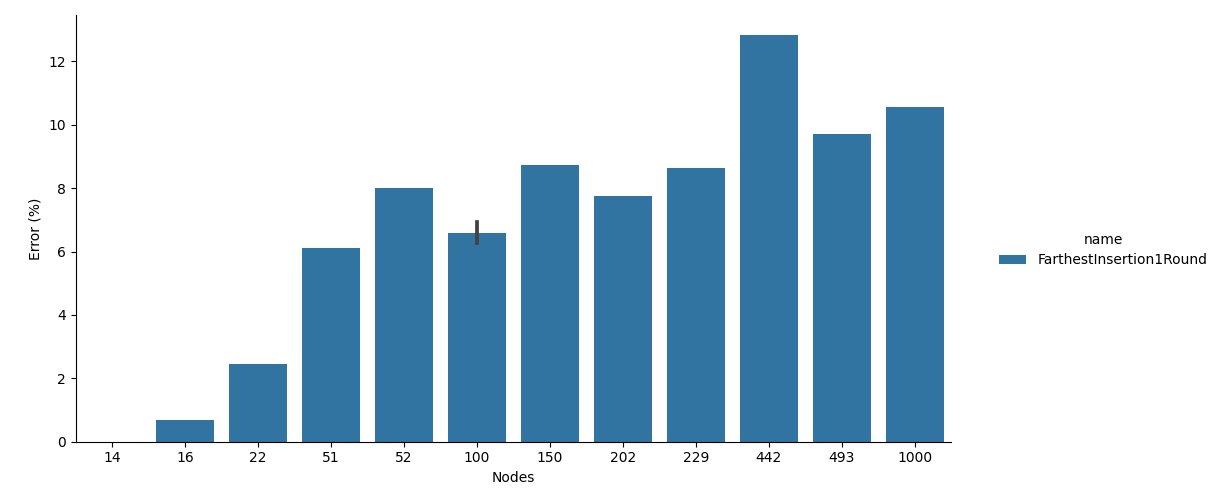
\includegraphics[width=0.9\textwidth]{./images/FarthestInsertion1Round__approximation_error_.png}

    \caption{Errore introdotto da FarthestInsertion rispetto al numero di nodi}
    \label{fig:farthest-insertion-accuracy-error}
\end{figure}

\noindent È doveroso mostrare le differenze tra Closest Insertion e
Farthest Insertion data la dualità delle due euristiche. Come
illustrato dal grafico
\ref{fig:closest-farthest-insertion-accuracy-error}, Farthest
Insertion approssima meglio il problema introducendo meno errore.\\

\begin{figure}[H]
    \centering

    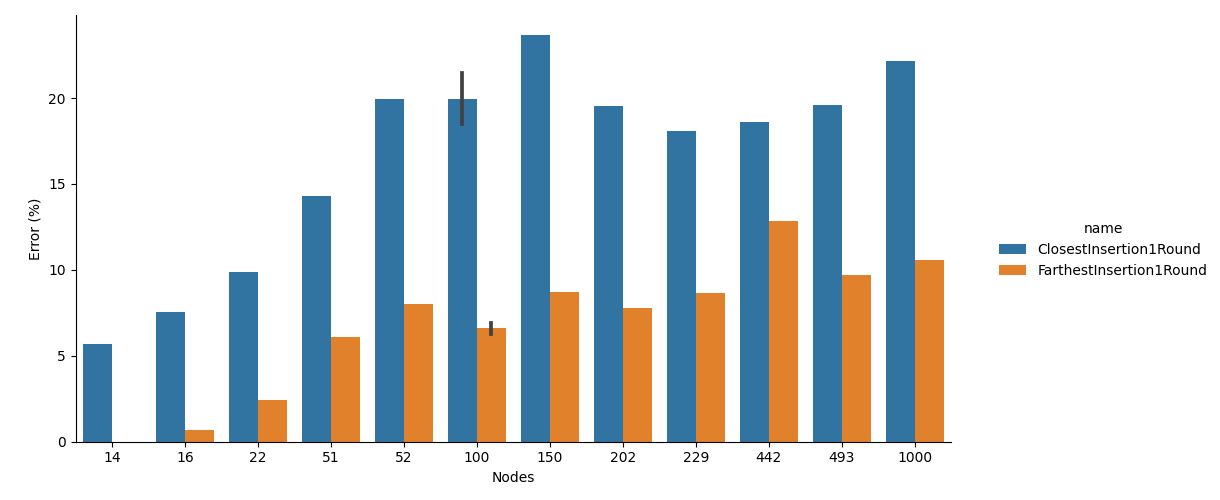
\includegraphics[width=0.9\textwidth]{./images/ClosestInsertion1Round_vs_FarthestInsertion1Round__approximation_error_.png}

    \caption{Confronto dell'errore introdotto da Closest Insertion e Farthest Insertion rispetto al numero di nodi}
    \label{fig:closest-farthest-insertion-accuracy-error}
\end{figure}

\noindent Anche per l'esecuzione con più round paralleli (meccanismo descritto
in \ref{sec:rounds}), nonostante il grafico evidenzi un leggero cambiamento dei dati, Farthest Insertion continua ad essere migliore. Si veda il grafico
\ref{fig:closest-farthest-insertion-4-rounds-accuracy-error}.\\

\begin{figure}[H]
    \centering

    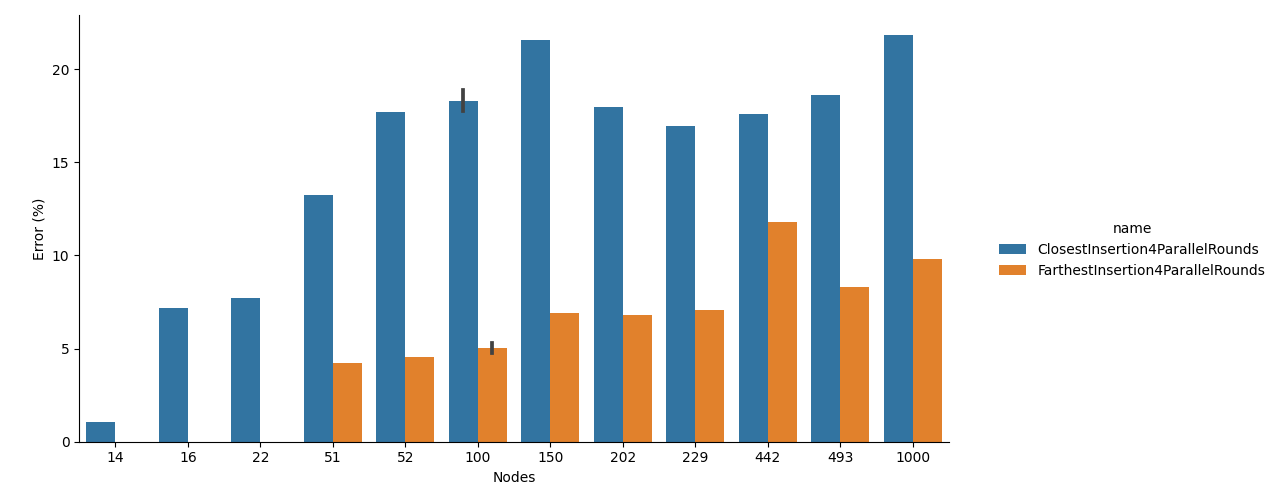
\includegraphics[width=0.9\textwidth]{./images/ClosestInsertion4ParallelRounds_vs_FarthestInsertion4ParallelRounds__approximation_error_.png}

    \caption{Confronto dell'errore introdotto da ClosestInsertion e FarthestInsertion su 4 rounds rispetto al numero di nodi}
    \label{fig:closest-farthest-insertion-4-rounds-accuracy-error}
\end{figure}

\subsection{Round paralleli di algoritmi euristici sequenziali}
\label{sec:rounds}

\noindent Le euristiche costruttive come Closest Insertion (descritta alla sezione
\ref{sec:closest-insertion}) e Farthest Insertion (descritta alla
sezione \ref{sec:farthest-insertion}) prevedono un'inizializzazione
deterministica del problema, scegliendo sempre il vertice
$0$ come primo nodo. Tuttavia, dando la possibilità di scegliere nodi sorgenti diversi, le soluzioni ritornati dall'algoritmo potrebbero differire e molteplici esecuzioni dell'algoritmo con nodi di partenza diversi scelti arbitrariamente potrebbero produrre soluzioni più
accurate rispetto ad una singola esecuzione partendo da un nodo fissato.\\

\noindent Abbiamo deciso di sfruttare questo fatto eseguendo più volte in parallelo l'algoritmo sequenziale con nodo iniziale casuale, e restituendo la migliore soluzione tra quelle ottenute. \\

\noindent Agli algoritmi è infatti passato un
\mintinline{c++}{RandomGenerator} che consente di generare un numero
casuale, rappresentante la sorgente del ciclo Hamiltoniano da
costruire. In realtà, il random generator è fornito in diverse
implementazioni:
\begin{itemize}
    \item \mintinline{c++}{RealRandomGenerator}, generatore per numeri
      casuali di tipo reale;
    \item \mintinline{c++}{IntegerRandomGenerator}, generatore per
      numeri casuali di tipo intero;
    \item \mintinline{c++}{FixedGenerator}, generatore del numero
      specificato al momento della creazione del generator.
\end{itemize}

\noindent L'inizializzazione può quindi differire in base al generator fornito
in input: se il generator è un \mintinline{c++}{FixedGenerator} allora
la sorgente scelta è fissata (come mostrato a lezione), fornendo così la versione base
dell'algoritmo che non ha bisogno di molteplici esecuzioni per
restituire il risultato, altrimenti la sorgente è scelta in modo
casuale.\\

\noindent Nel nostro caso abbiamo eseguito l'algoritmo prima con
sorgente fissata a $0$ e poi con sorgente random e fissando il numero
di istanze parallele a $4$ (numero di core disponibili): i risultati dell'esecuzione parallela con nodi di partenza casuali
sono stati soddisfacenti, infatti come si può notare dai grafici
\ref{fig:closest-insertion-1-4-rounds-accuracy-error} e
\ref{fig:farthest-insertion-1-4-rounds-accuracy-error}, più esecuzioni
dell'algoritmo tendono a restituire soluzioni più corrette.\\

\begin{figure}[!ht]
    \centering

    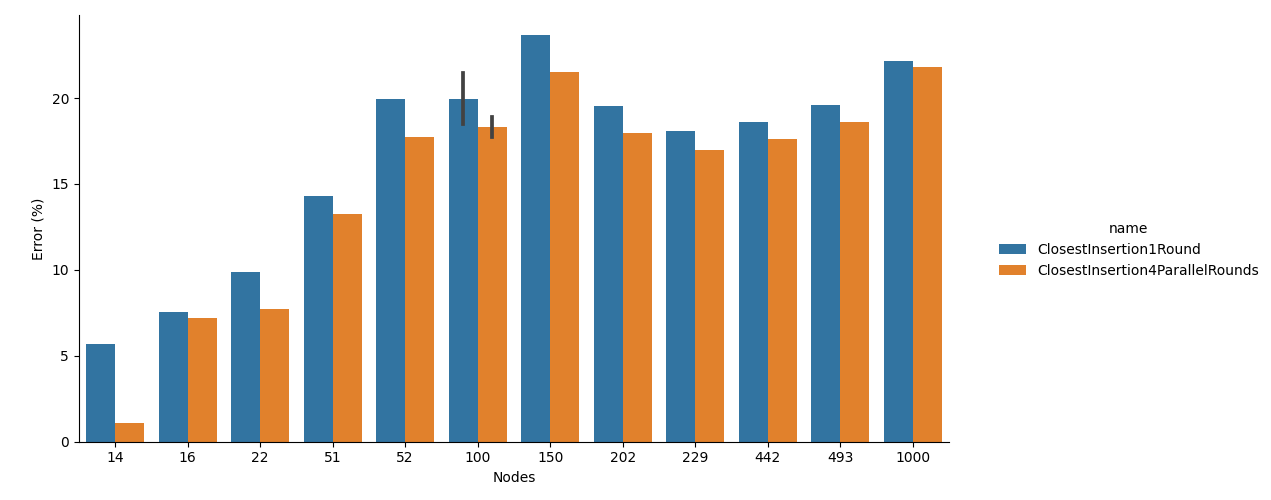
\includegraphics[width=0.9\textwidth]{./images/ClosestInsertion1Round_vs_ClosestInsertion4ParallelRounds__approximation_error_.png}

    \caption{Confronto dell'errore introdotto da ClosestInsertion con 1 round e con 4 rounds rispetto al numero di nodi}
    \label{fig:closest-insertion-1-4-rounds-accuracy-error}
\end{figure}

\begin{figure}[!ht]
    \centering

    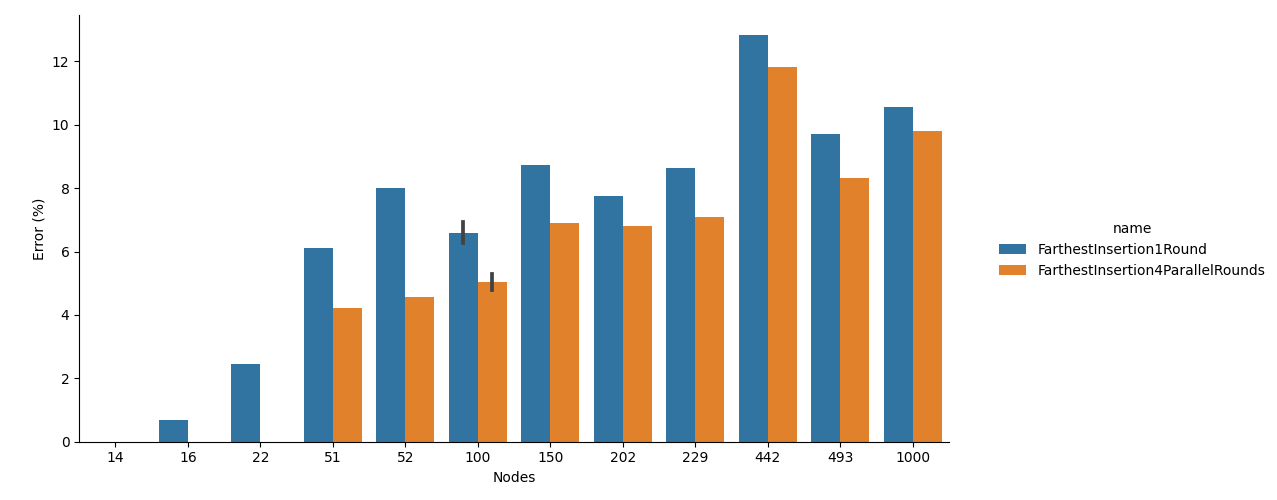
\includegraphics[width=0.9\textwidth]{./images/FarthestInsertion1Round_vs_FarthestInsertion4ParallelRounds__approximation_error_.png}

    \caption{Confronto dell'errore introdotto da FarthestInsertion con 1 round e con 4 rounds rispetto al numero di nodi}
    \label{fig:farthest-insertion-1-4-rounds-accuracy-error}
\end{figure}

\subsection{Farthest Insertion Alternativo}
\label{alg:farthest-insertion-alt}

Il progetto \codeinline{FarthestInsertionAlternative} contiene
un'implementazione alternativa dell'euristica costruttiva Farthest
Insertion per risolvere il problema del TSP metrico. L'algoritmo è
tratto da \textit{Cook et al.}\footnote{\url{https://onlinelibrary.wiley.com/doi/10.1002/9781118033142.ch7}}
e prevede i seguenti step:

\begin{enumerate}
    \item Inizializzazione: considera i due vertici $u$ e $v$ che
      compongono l'arco di costo maggiore;
    \item Selezione: trova un vertice $k$ non presente nel circuito
      parziale $C$ che massimizza $\delta(k,C)$;
    \label{pseudo:farthest-insertion-alt-selection}
    \item Inserimento: trova l’arco ${i, j}$ del circuito parziale che
      minimizza il valore $w(i, k) + w(k, j) - w(i, j)$ e lo inserisce
      $k$ tra $i$ e $j$;
    \item ripete da \ref{pseudo:farthest-insertion-alt-selection}
      finché non ha inserito tutti i vertici nel circuito.
\end{enumerate}

\noindent Rispetto all'algoritmo descritto alla sezione
\ref{sec:farthest-insertion}, cambia solo il primo step. La
complessità resta quindi $\bigO{n^2}$. \\

\noindent I risultati ottenuti da questo algoritmo sono illustrati dai grafici
\ref{fig:farthest-insertion-alt-accuracy-error} e
\ref{fig:farthest-insertion-alt-vs-std-1-4-rounds-accuracy-error}.
Dal secondo grafico possiamo notare che rispetto alla versione
standard (con un solo round) questo algoritmo si comporta un po'
meglio su taglie piccole dell'input, peggiorando invece su taglie più
grosse, mentre nella versione a 4 round (eseguiti su una CPU quad core in parallelo) è l'algoritmo che commette meno errori in 5 casi su 12.
a competere in quasi nessun caso.

\begin{figure}[!ht]
    \centering

    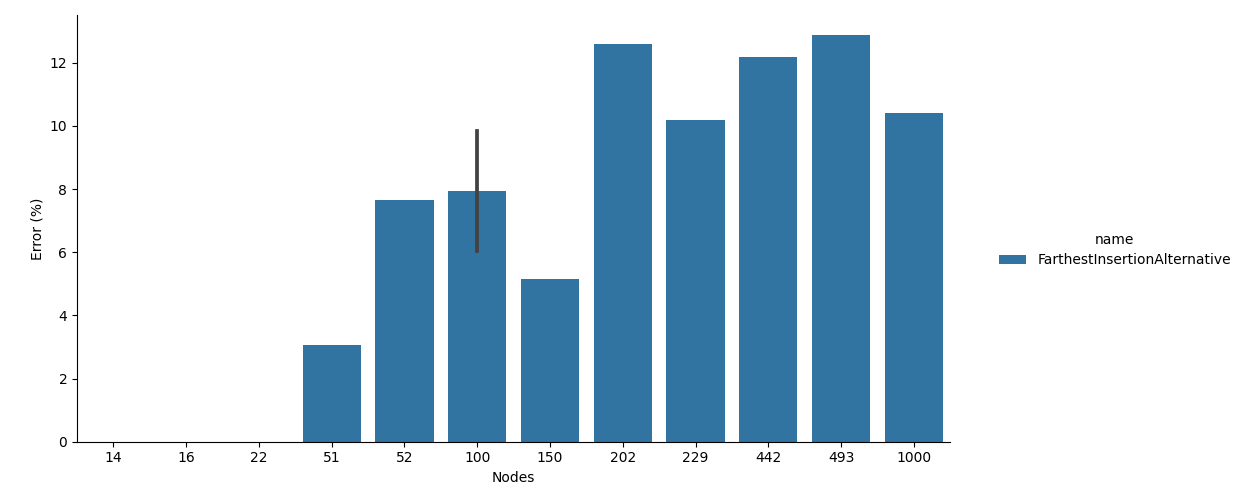
\includegraphics[width=0.9\textwidth]{./images/FarthestInsertionAlternative__approximation_error_.png}

    \caption{Errore introdotto da FarthestInsertionAlternative rispetto al numero di nodi}
    \label{fig:farthest-insertion-alt-accuracy-error}
\end{figure}

\begin{figure}[!ht]
    \centering

    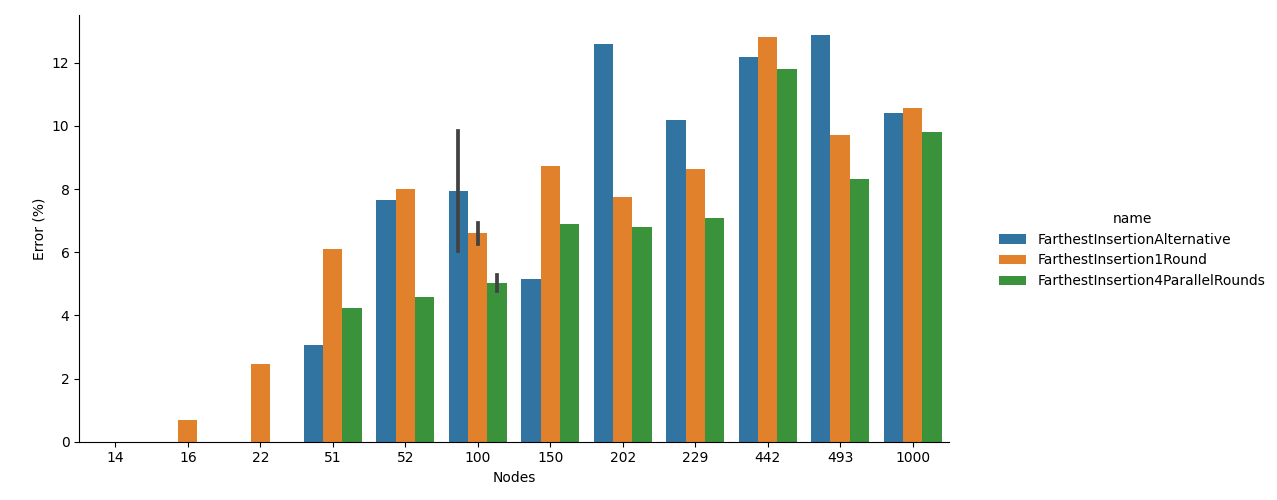
\includegraphics[width=0.9\textwidth]{./images/FarthestInsertionAlternative_vs_FarthestInsertion1Round_vs_FarthestInsertion4ParallelRounds__approximation_error_.png}

    \caption{Confronto dell'errore introdotto da FarthestInsertionAlternative e FarthestInsertion ``standard'' rispetto al numero di nodi}
    \label{fig:farthest-insertion-alt-vs-std-1-4-rounds-accuracy-error}
\end{figure}

\subsection{TSP con Simulated Annealing}

\subsubsection{Metodo Generale}

% TODO: tagliare un po' questo paragrafo
% Simulated Annealing è un metodo di ricerca stocastico proveniente dalla Meccanica Statistica che modella lo spazio di ricerca delle soluzioni emulando il processo fisico di \textit{annealing}. L'annealing è il processo con cui un solido, portato allo stato liquido tramite riscaldamento ad alte temperature, viene portato nuovamente allo stato solido, controllando e riducendo gradualmente la temperatura. Intuitivamente, ad alte temperature gli atomi del sistema sono in uno stato altamente disordinato: l'energia del sistema è massima.
% Per riportare tali atomi in una configurazione statisticamente molto ordinata (energia minima), la temperatura del sistema deve essere gradualmente abbassata. Riduzioni di temperature troppo drastiche provocano stress termico, che rovina il sistema stesso.

\noindent Simulated Annealing è un metodo di ricerca stocastico in cui l'abilità di superare minimi locali è governata da un parametro di controllo detto "temperatura". Quando la temperatura è elevata, Simulated Annealing è simile ad una ricerca casuale di una soluzione, mentre a temperature basse, quando la temperatura è molto vicina a 0, l'algoritmo si comporta similmente a Gradient Descent e resta intrappolato nel minimo locale più vicino. \\

\noindent La temperatura è inizialmente alta, il che corrisponde ad un'alta probabilità di accettare transizioni a soluzioni non migliorative, ed è ridotta gradualmente nel tempo. La policy di raffreddamento è regolata da un altro parametro di controllo, ed emula il processo fisico di annealing, in cui un materiale solido è scaldato fino a passare allo stato liquido (dove l'energia degli atomi è massima), per essere raffreddato gradualmente per assumere una struttura cristallina (dove gli atomi tornano in uno stato di massimo ordine, e la loro energia è quindi minima). \\

\noindent Come altri metodi di ricerca stocastici, Simulated Annealing esplora l'universo di possibli soluzioni perturbando iterativamente una soluzione iniziale; a differenza di molti metodi, però, la temperatura dell'algoritmo permette di accettare anche soluzione peggiorative, il che aiuta ad evitare la convergenza in un minimo locale. \\

\noindent Ad ogni iterazione, Simulated Annealing seleziona una soluzione "vicina" alla soluzione corrente. Se la nuova soluzione ha un costo (chiamato \textit{fitness}) migliore della precedente, è sempre accettata come nuova soluzione corrente. Se invece la nuova soluzione ha un fitness peggiore, essa è accettata con una certa probabilità (legata alla distribuzione di Boltzmann). Tale probabilità è dipendente rispetto alla differenza $\Delta E$ tra le fitness delle due soluzioni confrontate e rispetto alla temperatura corrente. La probabilità di accettare soluzioni peggiorative decresce mano a mano che la temperatura diminuisce e l'ordine di grandezza di $\Delta E$ aumenta.

\noindent Abbiamo deciso di implementare Simulated Annealing perché:

\begin{itemize}
    \item Spesso converge a soluzioni sufficientemente vicine alla soluzione ottima in brevissimo tempo;
    \item È stato studiato per molti anni e la ricerca ha prodotto estensioni e miglioramenti rispetto all'algoritmo originale;
    \item Alcune varianti di Simulated Annealing sono già state applicate con successo a casi particolare di TSP, come ad esempio \textit{Compressed Annealing} per risolvere \textit{Traveling Salesman Problem with Time Windows};
    \item Se si usa Random Restart, è facile da parallelizzare;
    \item È un algoritmo citato nel corso di Intelligenza Artificiale, ma prima d'ora non avevamo mai avuto l'occasione di implementarlo e osservarlo in pratica.
\end{itemize}

\noindent I suoi punti di debolezza, invece, sono:

\begin{itemize}
    \item È non deterministico ed è difficile prevedere quanto la soluzione ritornata possa essere peggiore della soluzione ottima;
    \item Se la temperatura iniziale non è inizializzata correttamente rispetto all'input atteso, le performance dell'algoritmo degradano e le soluzioni ritornate possono essere molto distanti da quella ottima.
    \item Se la temperatura viene raffreddata troppo velocemente, le performance degradano similmente al punto precedente.
    \item Se le dimensioni degli input dell'algoritmo differiscono molto e i parametri di Simulated Annealing sono fissati, è difficile ottenere buoni risultati su tutte le istanze di input.
\end{itemize}

\subsubsection{Scelta della soluzione iniziale}

Simulated Annealing richiede una soluzione di partenza, la quale sarà poi iterativamente sottoposta a perturbazioni per esplorare soluzioni vicine. Nel nostro caso, abbiamo deciso di usare l'euristica \textbf{Nearest Neighbors}. Le regioni per questa scelta sono:

\begin{itemize}
    \item È molto veloce e la soluzione ritornata non è troppo distante dalla soluzione ottima di TSP;
    \item È una tra le euristiche costruttive proposte nell'homework che non abbiamo implementato come metodo a sé, ed eravamo curiosi di implementarla.
\end{itemize}

Per essere ragionevolmente sicuri di partire da una buona soluzione iniziale, Nearest Neighbors è lanciato 10 volte. Di queste 16 esecuzioni, la soluzione selezionata è il circuito Hamiltoniano ritornato di peso minore.

\subsubsection{Scelta delle soluzioni vicine}

Il criterio di selezione di Simulated Annealing è strettamente dipendente al problema a cui è applicato. Nel caso di TSP, abbiamo deciso di generare perturbazioni in 3 modi diversi ispirati alla ricerca euristica di Lin-Kernighan\footnote{\url{https://arxiv.org/pdf/1003.5330.pdf}}, di cui solo uno di essi è scelto casualmente ad ogni iterazione. \\

\noindent Questi metodi condividono lo stesso setup iniziale, definito nella metodo \codeinline{TSPSolution::manipulate\_raw} in \codeinline{SimulatedAnnealing/TSPSolutionPool.h}:

\begin{itemize}
    \item Vengono selezionati casualmente due indici del circuito Hamiltoniano corrente $x, y$ tali che $x < y$ e che $x > 0$, $y < n - 1$;
    \item Viene estratto un valore a caso $d \in [0, 1]$;
    \item Se $0 < d < 0.4$, viene eseguito uno step \textit{2-opt};
    \item Se $0.4 \leq d < 0.8$, viene eseguito uno step \textit{translate};
    \item Se $0.8 \leq d \leq 1$, viene eseguito uno step \textit{switching}.
\end{itemize}

\noindent Chiamiamo $\pi$ il circuito Hamiltoniano attuale e $\pi'$ una perturbazione di tale circuito che preserva la proprietà di essere un circuito Hamiltoniano dello stesso insieme di nodi.

\paragraph{2-opt}\mbox{}\\

\begin{enumerate}
    \item Vengono copiati i primi $x$ elementi di $\pi$ in $\pi'$;
    \item I successivi $x$ elementi di $\pi$ sono copiati in ordine inverso;
    \item Viene copiata l'ultima parte di $\pi$ in $\pi'$.
\end{enumerate}

\paragraph{Translate}\mbox{}\\

\begin{enumerate}
    \item Vengono copiati i primi $x$ elementi di $\pi$ in $\pi'$;
    \item Viene copiato l'elemento $\pi[y-1]$ in $\pi'$;
    \item Vengono copiati i successivi $y - x - 1$ elementi di $\pi$ in $\pi'$;
    \item Viene copiata l'ultima parte di $\pi$ in $\pi'$.
\end{enumerate}

\paragraph{Swithing}\mbox{}\\

\begin{enumerate}
    \item Vengono copiati i primi $x$ elementi di $\pi$ in $\pi'$;
    \item Viene copiato l'elemento $\pi[y-1]$ in $\pi'$;
    \item Saltando l'elemento $\pi[x]$, vengono copiati i successivi $y - x - 2$ elementi di $\pi$ in $\pi'$;
    \item Viene copiato l'elemento $\pi[x]$ in $\pi'$;
    \item Viene copiata l'ultima parte di $\pi$ in $\pi'$.
\end{enumerate}

\subsubsection{Scelta della temperatura iniziale}

Inizialmente avevamo fissato la temperatura inizale a $1.000.000$. Questa scelta sembrava funzionare per la maggiorparte dei dataset dell'homework, ma ci siamo accorti che le performance degradavano di molto per grafi con più di 150 nodi. \\

\noindent Abbiamo quindi adottato il metodo di inizializzazione di Ben-Ameur\footnote{\url{https://www.researchgate.net/publication/227061666_Computing_the_Initial_Temperature_of_Simulated_Annealing}}, che si basa sul coefficiente di accettazione iniziale $\chi{}_0$. $\chi{}_0$ rappresenta la percentuale di transizioni sfavorevoli di simulated annealing che ci aspettiamo vengano accettate alla prima iterazione dell'algoritmo. Solitamente il valore di $\chi{}_0$ è compreso nell'intervallo $[0.8, 0.\overline{99}]$. Nel nostro caso, $\chi{}_0 = 0.94$ ci ha dato i risultati medi migliori su tutti i dataset. \\

\noindent Per come abbiamo inizializzato i parametri del metodo di Ben-Ameur, grafi di dimensione più alta partiranno da una temperatura più alta, il che equivale ampliare il raggio di ricerca delle soluzioni all'aumentare della complessità dell'input.

\subsubsection{Reheating}

Una delle estensioni di Simulated Annealing prevede di riscaldare nuovamente la temperatura dopo un certo numero di iterazioni. L'intuizione è che questo dà la possibilità di ampliare lo spazio di ricerca delle soluzioni, e riduce maggiormente le possibilità che l'algoritmo converga in un minimo locale. \\

\noindent Nel nostro caso, la temperatura è aumentata ad intervalli regolari di valori via via decrescenti all'aumentare delle iterazioni di Simulated Annealing. La formula di reheating è la seguente, dove $\tau{}$ è la temperatura corrente, $\tau{}_0$ è la temperatura iniziale, $i$ è l'iterazione corrente, $\rho$ è il fattore di reheating:

\begin{equation}
    \tau{} = \frac{\tau{}_0 \cdot \rho{}}{10 \cdot (i + 1)}
\end{equation}

L'ampiezza degli intervalli di \textit{reheating} è fissata e data dalla seguente formula, dove $\tau{}_0$ rappresenta la temperatura iniziale:

\begin{equation}
    max\{ \frac{\tau{}_0}{4000}, 100 \}
\end{equation}

\noindent Tali formule sono state scelte in modo sperimentale, poiché non abbiamo trovato riferimenti a riguardo nella letteratura.

\subsubsection{Parallelismo}

Uno dei punti di forza di Simulated Annealing è che, se si applica Random Restart, l'algoritmo è banalmente parallelizzabile.
Random Restart consiste nel lanciare un algoritmo di ricerca stocastico (nel nostro caso, Simulated Annealing) un certo numero di volte, restituendo solamente la migliore soluzione trovata. \\

\noindent Abbiamo definito la classe di utilità \codeinline{parallel\_executor} in \codeinline{Shared/parallel.h}, la quale si occupa di eseguire una funzione \textit{higher-order} su un certo numero di thread paralleli e di selezionare la migliore soluzione ottenuta. Essa è stata utilizzata per eseguire in parallelo molteplici istanze indipendenti di Simulated Annealing. In particolare, il numero di istanze eseguite in parallelo è par al numero di core fisici della CPU del computer di esecuzione.

\subsubsection{Steady Steps}

\noindent Per evitare il rischio di abbassare la temperatura del sistema troppo velocemente, e per esplorare un maggior numero di possibili soluzioni, l'algoritmo genera un numero costante di soluzioni vicine rispetto alla soluzione corrente prima di effettuare un passo di annealing (che consiste nel moltiplicare la temperatura corrente per il coefficiente di raffreddamento $\beta$). \\

\noindent Abbiamo determinato sperimentalmente che un buon numero di \textit{steady steps} è 5.

\subsubsection{Criterio di convergenza}

\noindent Nella letteratura sono presenti diversi criteri per determinare quando Simulated Annealing ha effettuato un numero sufficiente di iterazione. Per cercare di garantire una certa robustezza alla nostra implementazione, ne abbiamo applicati diversi:

\begin{itemize}
    \item \textbf{Massimo numero di iterazioni}: è il criterio più semplice, consiste nel fermarsi una volta superato un certo numero predefinito di \textit{annealing steps};
    \item \textbf{Raggiungimento temperatura minima}: l'algoritmo si ferma la temperatura ha raggiunto un valore prossimo a 0. Noi consideriamo $1 \cdot 10^{-16}$ come temperatura minima;
    \item \textbf{Miglior soluzione ripetuta}: la ricerca si ferma se la miglior soluzione individuata non cambia per un certo numero di iterazioni consecutive. Noi consideriamo fino a $150$ ripetizioni consecutive della stessa migliore soluzione prima di dichiarare la convergenza.
\end{itemize}

\noindent Le condizioni precedentemente elencate sono trattate in modo
disgiunto, ovvero l'algoritmo termina non appena si verifica almeno
una delle condizioni di convergenza.
